\documentclass[11pt]{article}
\usepackage[margin=1in]{geometry}
\usepackage{graphicx,booktabs,amsmath,hyperref}
\title{HST ACS/WFC Two-Axis CTE Trail Audit}
\author{Biswajit Jana}
\date{\today}
\begin{document}
\maketitle

\begin{abstract}
This is a reproducible, bounded audit of charge-transfer-efficiency (CTE) trail
suppression in calibrated Advanced Camera for Surveys / Wide Field Channel
(ACS/WFC) products. It compares serial- and parallel-axis trail profiles
between CTE-uncorrected (FLT) and pixel-based CTE-corrected (FLC) products for
the same exposures, as a function of source charge, background level, and
parallel transfer distance. It is an independent archive-product verification;
it is not a replacement for CALACS or a new PCTETAB. The synthetic
injection-recovery validation gate (Section~\ref{sec:validation}) passed. On a
small, deterministic real-data sample (3 ACS/WFC F606W exposure pairs, public
HST proposal 18004; Section~\ref{sec:results}), the median trail-charge
suppression fraction across $n=36$ sources was $0.79$, consistent with
substantial but incomplete removal of parallel CTE trails by the pixel-based
correction; per-source scatter is large and this bounded sample is not a
statement about ACS/WFC performance in general (Section~\ref{sec:limitations}).
\end{abstract}

\section{Scientific question}
How effectively do current ACS/WFC calibrated products suppress serial and
parallel charge-transfer trails across source charge, background and
transfer distance?

\section{Data and provenance}
\label{sec:data}
The real-data sample is drawn from HST proposal 18004 (PI: Matthew Hayes),
ACS/WFC filter F606W, calibration level 2 (FLT/FLC), queried directly against
the MAST archive (\texttt{astroquery.mast.Observations}) and confirmed
\texttt{dataRights=PUBLIC} with no proprietary embargo. Three exposures were
selected deterministically (first 3 by sorted \texttt{obs\_id}):
\texttt{jfnx01mhq}, \texttt{jfnx01miq}, \texttt{jfnx01mkq}, yielding 6
FLT+FLC files ($\sim$964\,MB total). Exact product IDs, retrieval UTC
timestamps, SHA-256 checksums and data-use terms are recorded in
\texttt{data/manifest.csv} (see \texttt{docs/DATASET\_PLAN.md} and
\texttt{IMPLEMENTATION\_PLAN.md} for the selection criteria); raw FITS files
are not committed to the repository.

\section{Method}
Source detection uses \texttt{photutils.detection.DAOStarFinder} on a
sigma-clipped background-subtracted FLC image. For each detected source, a
1-D trail profile is extracted along the parallel (row) axis in the pixels
between the source and the readout amplifier, using a header-derived
geometry (\texttt{CCDAMP}/\texttt{CCDCHIP}; see
\texttt{docs/ASSUMPTIONS\_AND\_LIMITATIONS.md} for the explicit, documented
readout-corner convention). A buffer of \texttt{min\_distance=4} pixels
around the source excludes PSF-wing contamination. The trail is fit to a
single empirical exponential,
\[
  I(d) = A \exp(-d / L) + c,
\]
independently for FLT and FLC, via \texttt{scipy.optimize.curve\_fit}. Total
trailed charge is reported as the analytic integral $A \cdot L$, and
suppression is $1 - (A_{\mathrm{FLC}} L_{\mathrm{FLC}}) / (A_{\mathrm{FLT}}
L_{\mathrm{FLT}})$. This is the same descriptive functional form used in the
literature seeds (Anderson \& Bedin 2010; Massey et al. 2010), not a
multi-trap-species physical simulation. Hot/warm pixels are detected
independently via the DQ mask and cross-checked with a sigma-clipped
statistical detector.

\section{Validation and uncertainty}
\label{sec:validation}
Observational/statistical uncertainty is estimated via bootstrap resampling
(1000 resamples, 95\% confidence, seed 20260713, per
\texttt{config/analysis.yml}); numerical convergence uncertainty is assessed
separately via the fit covariance condition number and reduced
$\chi^2$ (\texttt{uncertainty.check\_fit\_convergence}), so the two sources
of uncertainty are never conflated.

The synthetic injection-recovery validation gate
(\texttt{tests/test\_trail\_profiles.py::test\_synthetic\_exponential\_trail\_recovery},
Figure~\ref{fig:injection}) injects a known exponential trail
(amplitude 1000\,e$^-$, length 6\,px on a 20{,}000\,e$^-$ source) into
labelled-synthetic data and recovers it via the full extraction+fit pipeline.
Across 15 independent noise realizations at this signal level, the observed
worst-case amplitude recovery error was 6.8\% and worst-case length recovery
error was 10.6\%; the automated test enforces a 15\%/25\% tolerance with
margin above that. \textbf{This gate passed}, so the fitting pipeline is
validated before being applied to real data. A null control
(\texttt{test\_null\_control\_zero\_trail\_amplitude\_consistent\_with\_zero})
confirms a flat, no-trail profile fits an amplitude consistent with zero.

\section{Results}
\label{sec:results}
All numbers below are read directly from \texttt{results/summary.json},
produced by \texttt{scripts/run\_analysis.py} on the real-data sample
described in Section~\ref{sec:data}; none are typed in by hand.

DAOStarFinder detected up to 40 candidate sources per exposure (120 total
across 3 exposures); after fitting and the physical-plausibility check on the
suppression fraction (Section~\ref{sec:validation}), $n=36$ sources yielded a
usable FLT/FLC trail-charge suppression measurement (84 candidates were
rejected --- ill-conditioned fits, non-converging optimizations, or
unphysical suppression values --- and recorded, not silently dropped, in
\texttt{results/warnings.json}). The median trail-charge suppression fraction
was $0.79$ ($n=36$). Binned by source charge (DAOStarFinder flux estimate,
3 quantile bins, $n\approx12$ each): mean suppression fraction $0.73$, $0.77$,
$0.40$ from faintest to brightest bin. Binned by parallel transfer distance
(3 quantile bins, $n\approx12$ each): $0.37$, $0.94$, $0.59$ from shortest to
longest transfer distance. Every bin is below the
\texttt{config/analysis.yml} \texttt{minimum\_sample\_size=30} threshold and
is flagged as such in \texttt{results/warnings.json}; these binned trends are
illustrative only, not independently significant at this sample size.
Independently, DQ-flagged hot pixels (ACS \texttt{HOTPIX}, DQ bit 16 --
verified against the CALACS source, \texttt{spacetelescope/hstcal},
\texttt{pkg/acs/include/acsdq.h}) showed a bootstrap mean excess of
$-5.5\,e^-$ (95\% CI $[-7.8, -3.4]$, $n=497{,}229$ pixels) relative to the
sigma-clipped image background; the negative sign is consistent with these
pixels already having their elevated dark current removed by dark
subtraction in the calibrated FLT product; see
Section~\ref{sec:limitations}.

\section{Limitations}
\label{sec:limitations}
An independent archive-product verification; not a replacement for CALACS or
a new PCTETAB. The real-data sample is 3 exposures from a single proposal,
filter and epoch; results here characterize this bounded sample, not ACS/WFC
performance in general. Per-source suppression-fraction scatter is large
(Figure~\ref{fig:charge}); the median is a robust summary but individual
sources --- including the one shown in Figure~\ref{fig:profiles} --- can show
no suppression or an apparently larger FLC trail than FLT, most plausibly
from photon-noise-dominated fits on faint sources rather than a real
correction failure. The hot-pixel excess measurement uses the whole flagged
population without separating pixels already corrected by dark subtraction
from residual anomalies. See \texttt{docs/ASSUMPTIONS\_AND\_LIMITATIONS.md}
for the full, explicit list of assumptions (readout-geometry convention,
trail model, PSF-buffer choice) and limitations (no local LaTeX compilation
check).

\section{Reproducibility}
\begin{verbatim}
python -m pip install -e ".[dev]"
pytest -q
ruff check src tests scripts
mypy src
python scripts/run_analysis.py --demo
python scripts/make_figures.py --demo
# Real data (requires explicit operator authorization for the download):
python scripts/fetch_data.py --i-have-authorization
python scripts/run_analysis.py
python scripts/make_figures.py
\end{verbatim}
Software version, git commit and configuration SHA-256 are recorded in
\texttt{results/summary.json} and each figure's sidecar JSON.

\begin{figure}
  \centering
  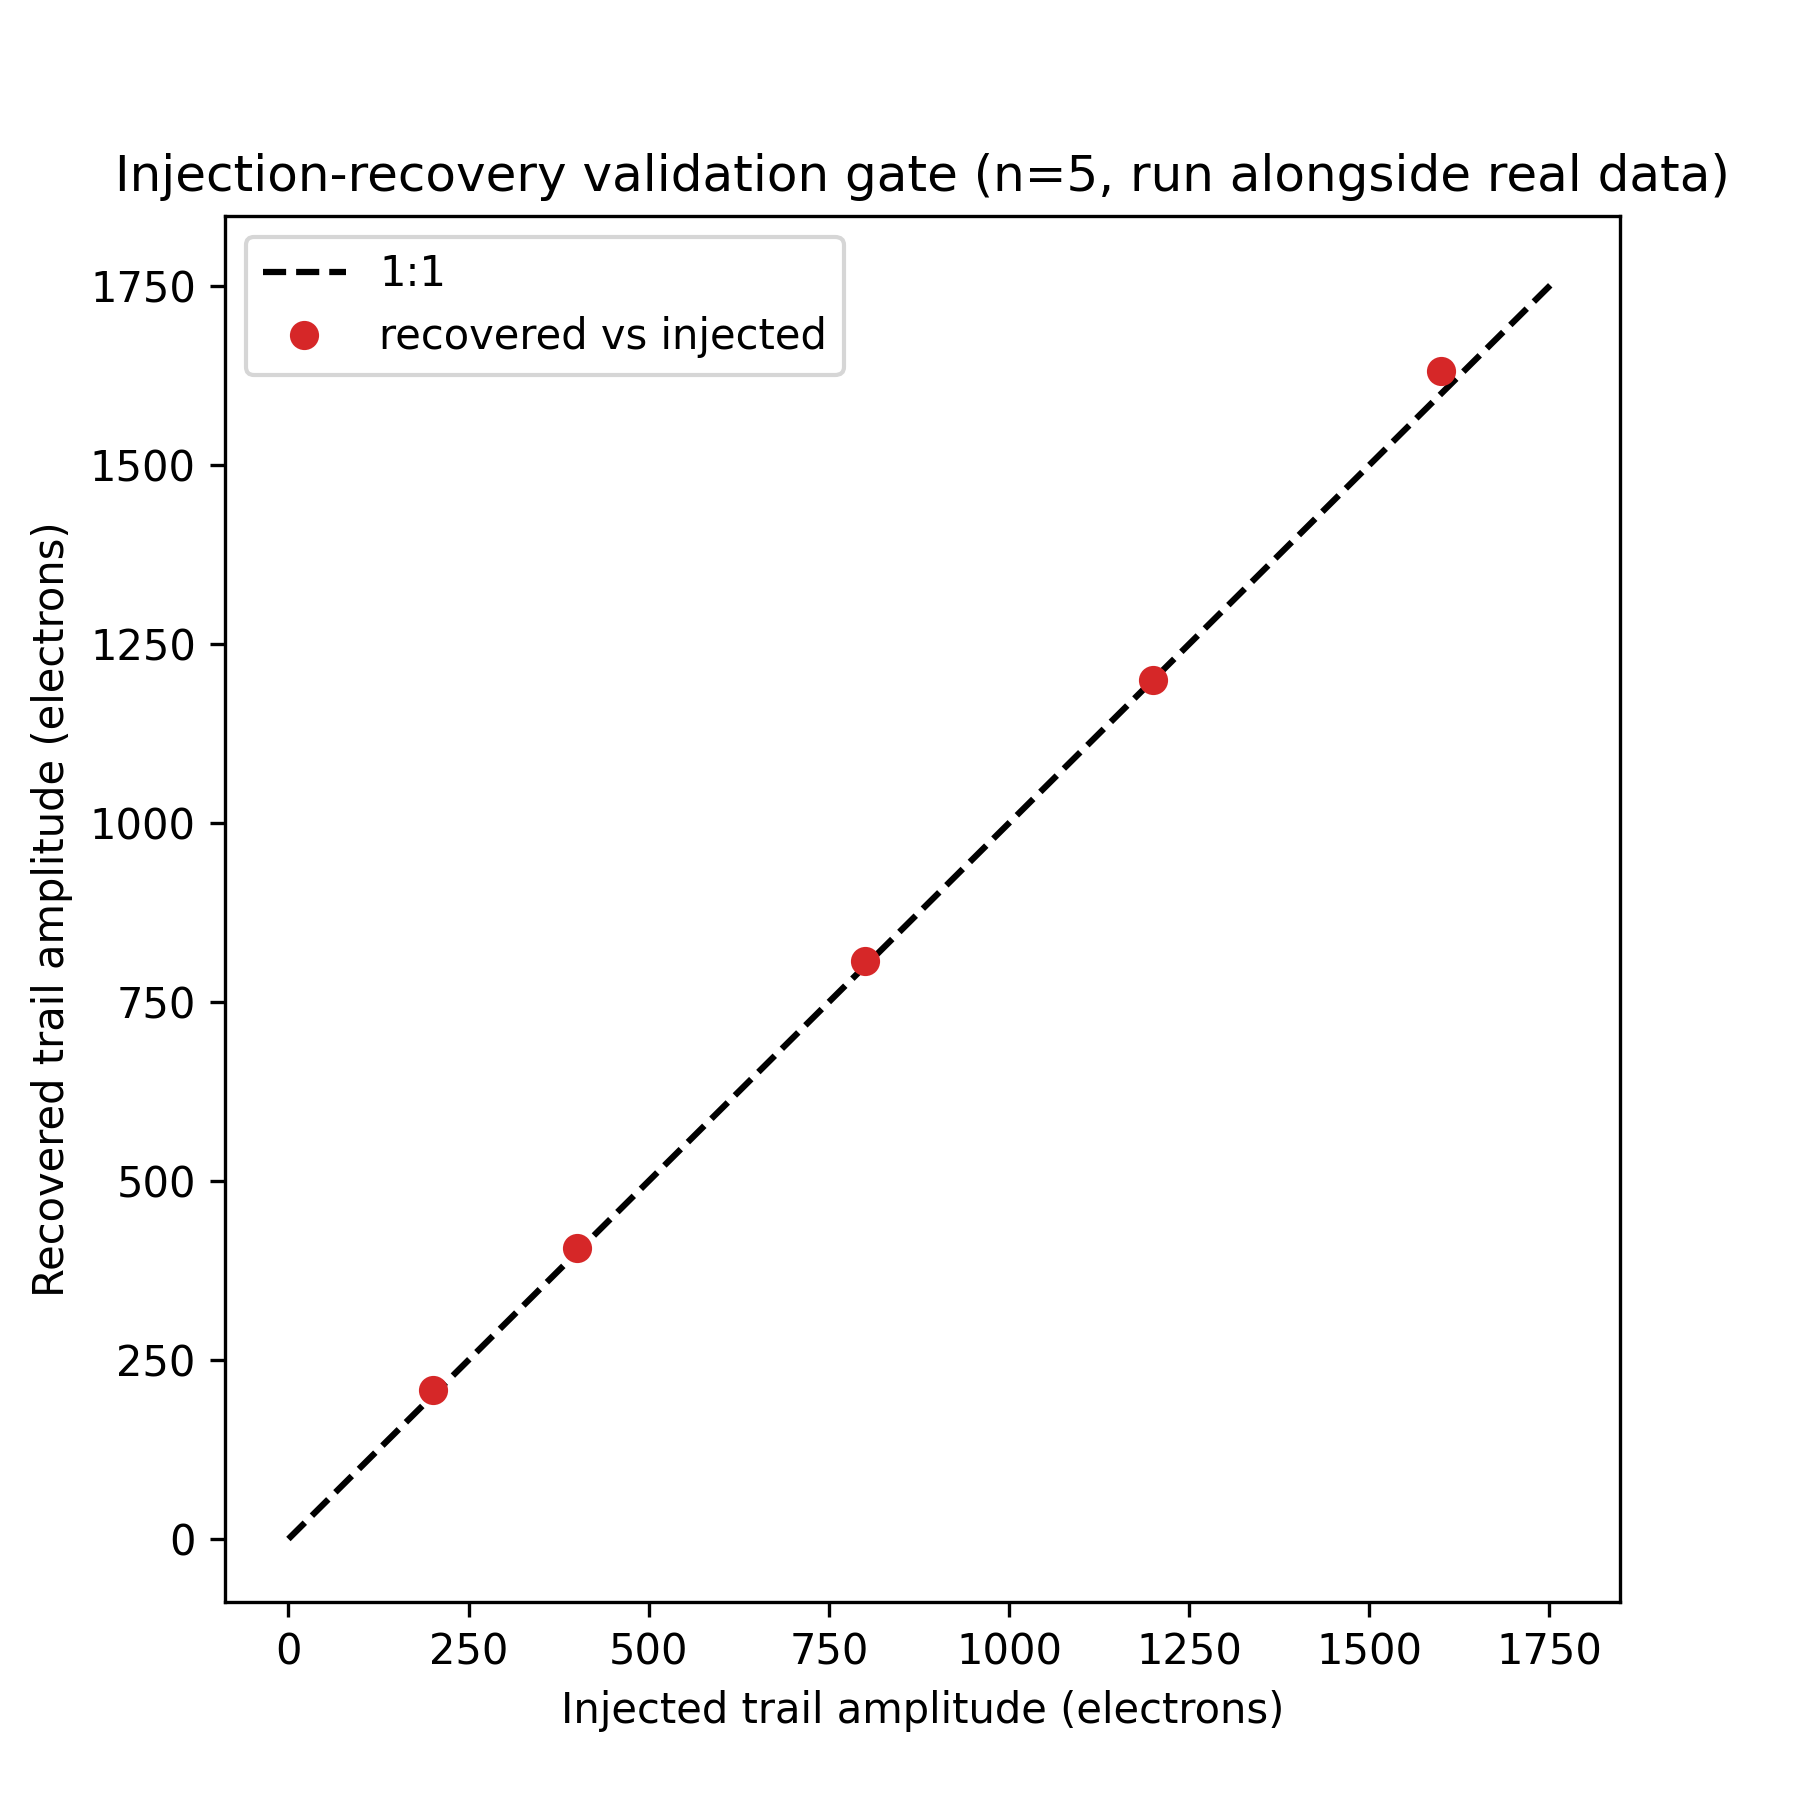
\includegraphics[width=0.8\textwidth]{../figures/fig06_injection_recovery.png}
  \caption{Synthetic injection-recovery validation: recovered vs injected
  trail amplitude, $n=5$ injected amplitudes. Points fall on the 1:1 line
  within the documented tolerance (Section~\ref{sec:validation}).}
  \label{fig:injection}
\end{figure}

\begin{figure}
  \centering
  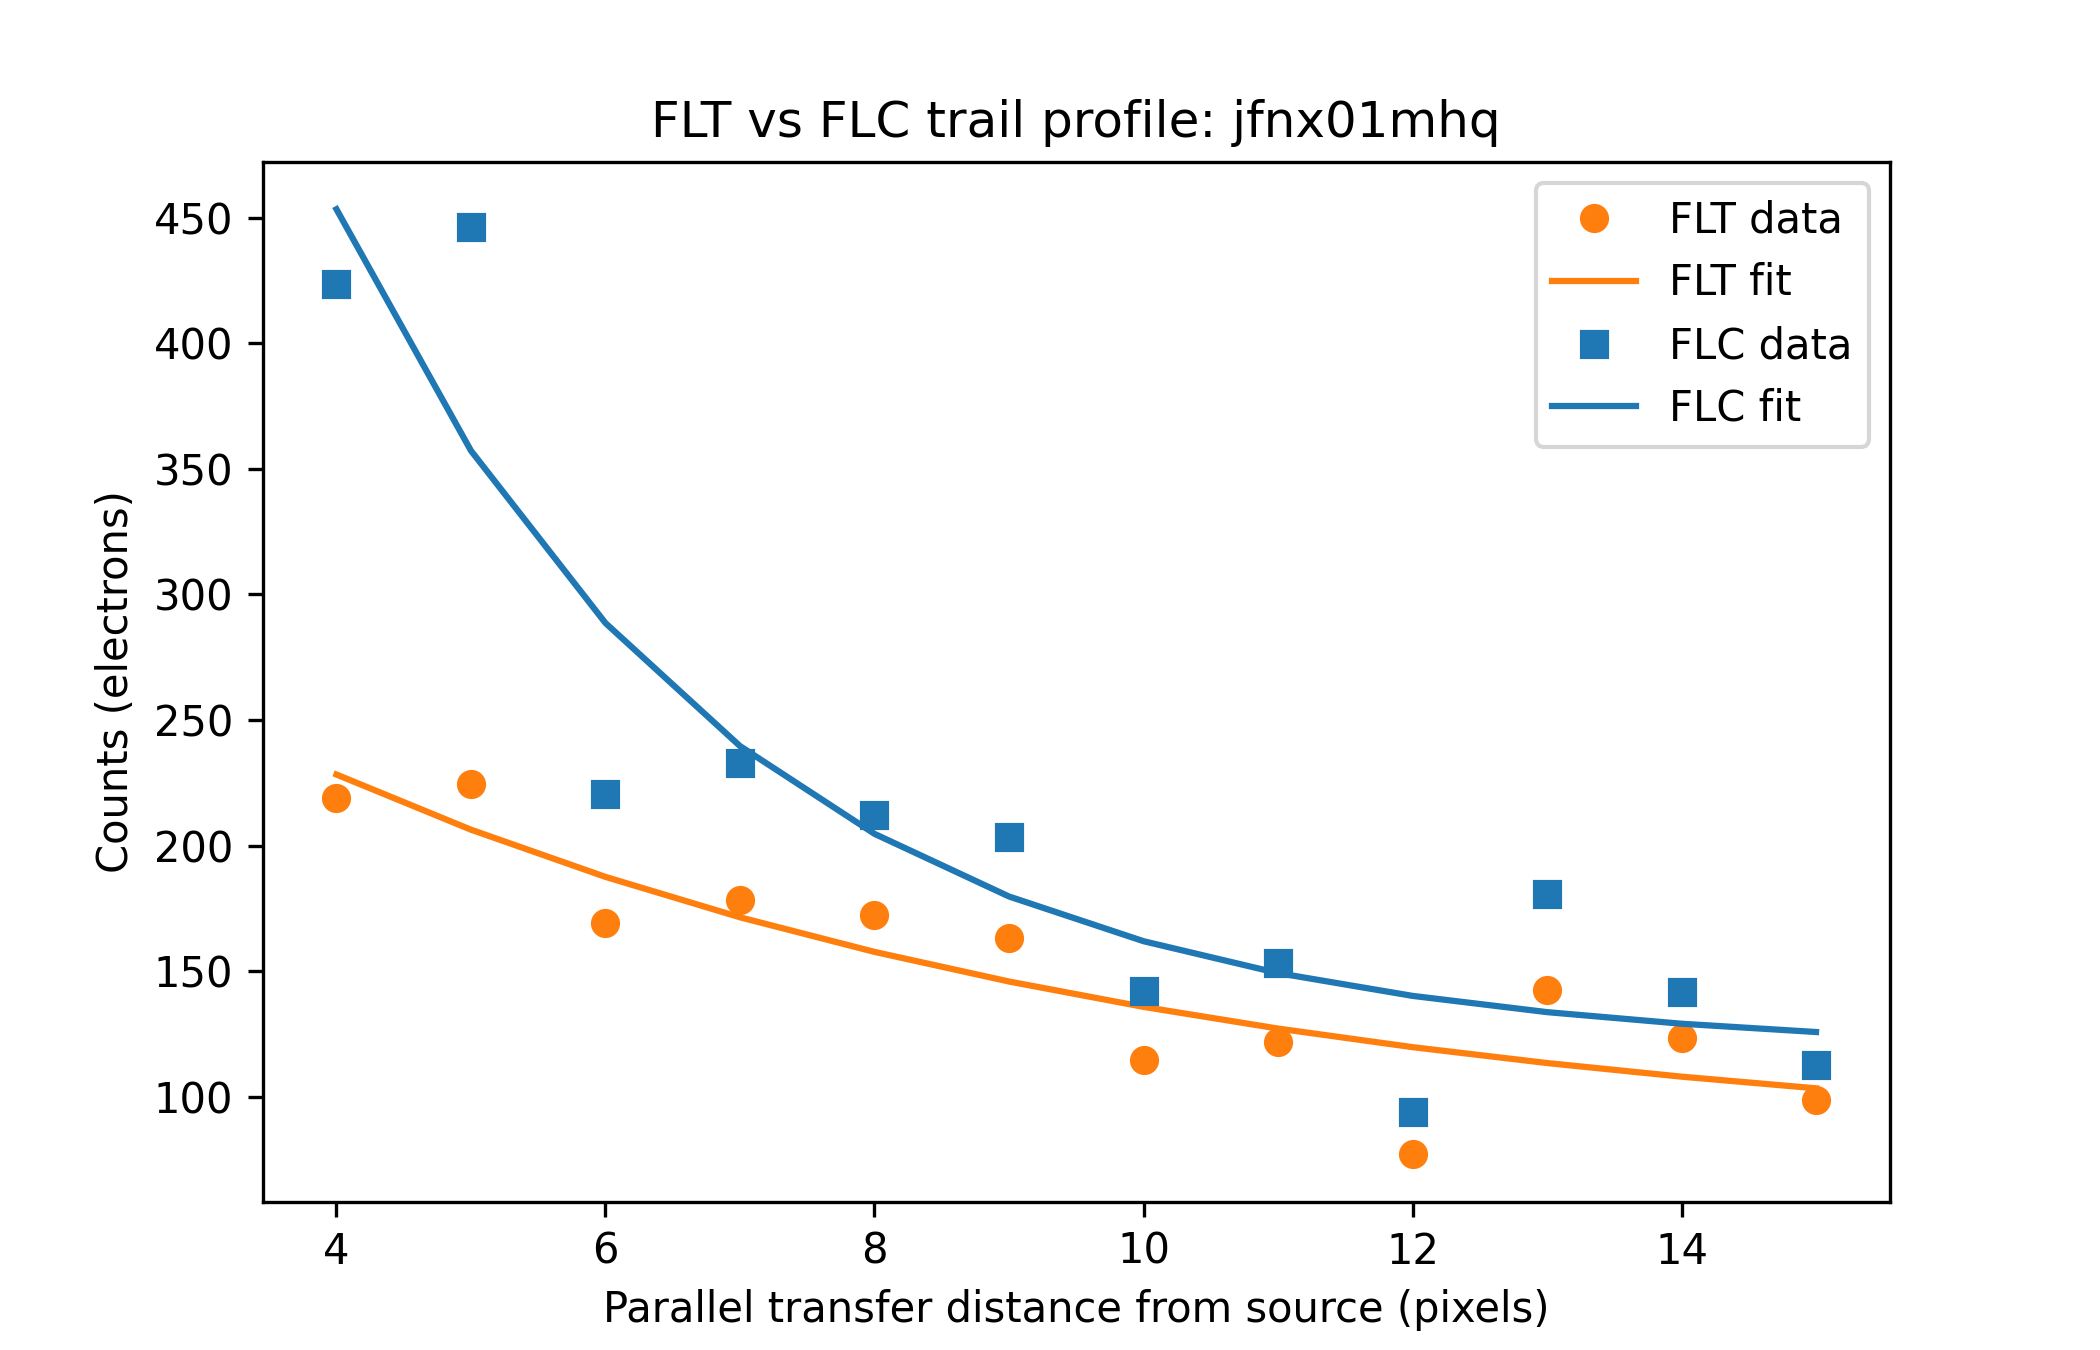
\includegraphics[width=0.8\textwidth]{../figures/fig03_flt_vs_flc_profiles.png}
  \caption{FLT vs FLC parallel trail profile for one real source in exposure
  \texttt{jfnx01mhq} (first of the 15 brightest candidates with a converging
  fit in both products). This particular source shows a larger FLC trail
  than FLT, illustrating the per-source scatter discussed in
  Section~\ref{sec:limitations}; it is not representative of the median
  behaviour across the full sample.}
  \label{fig:profiles}
\end{figure}

\begin{figure}
  \centering
  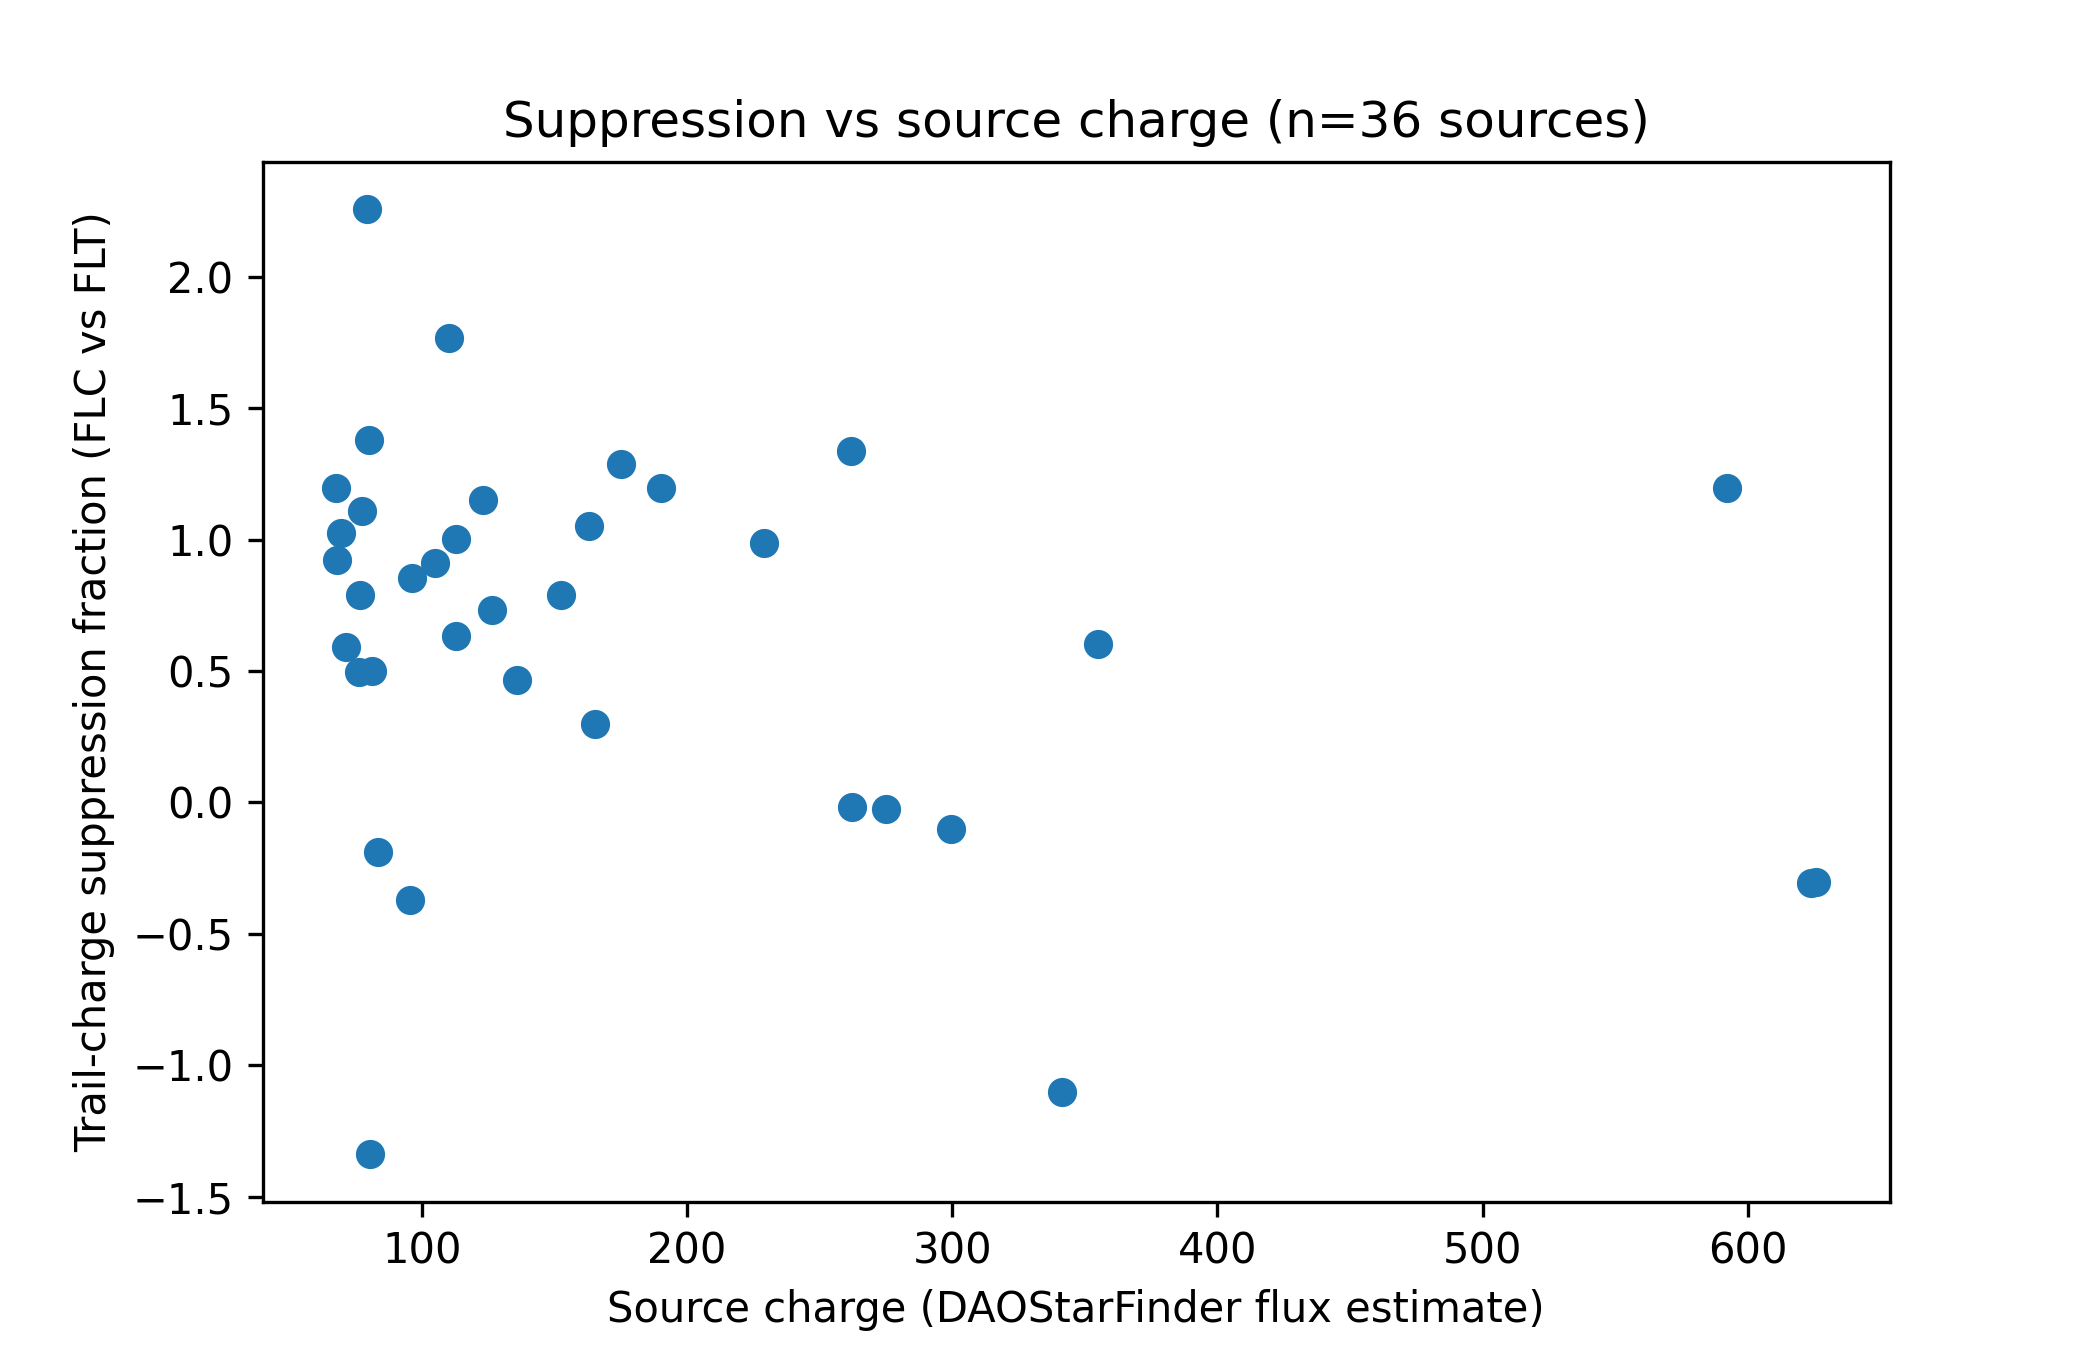
\includegraphics[width=0.8\textwidth]{../figures/fig04_suppression_vs_charge.png}
  \caption{Trail-charge suppression fraction vs source charge for all
  $n=36$ real sources passing the fit-quality and physical-plausibility
  checks (Section~\ref{sec:validation}). Scatter is large at this sample
  size; see Section~\ref{sec:results} for the binned means.}
  \label{fig:charge}
\end{figure}

\bibliographystyle{plain}
\bibliography{references}
\end{document}
